\section{Experimental Setup}
\label{sec:setup}
All experiments were conducted on our own machines, using a computer with an AMD Ryzen 9 5900X, 32 GB of RAM and an NVIDIA RTX 3090 GPU (10,496 CUDA cores, 1.70 GHz boost clock, 24 GB of GDDR6X memory, 35.58 TFlops) for resource-intensive workloads and our laptops for standard workloads and program refinement. We used four laptops: the two most powerful are a MacBook Air M3 and a machine with no dedicated GPU, 16 GB of RAM and an Intel Core i7-13700H.
For reproducibility, all environment settings have been documented and are available in the Bitbucket repository at \textit{https://bitbucket.org/upd-dei-stud-prj/seupd2526-retrix/src/master/} or can be reproduced by following the instructions in this paper.

\subsection{Dataset}
\label{sec:dataset}

The dataset consisted of 10,000 scientific publications that had to be paired with tweet-like posts written in three languages: German, French, and English. There are no explicit references such as URLs in any query. Instead, each tweet contains an implicit reference to a scientific paper, for example through mentions of authors or keywords related to the paper. The dataset files are all in JSON format. The scientific papers dataset contains the columns pubkey (unique identifier), title, abstract, venue/location and authors. The query datasets contain the columns index, pubkey (ID of the positive scientific paper that has to be matched with the query) and text.


\begin{table}[htbp]
	\centering
	\caption{Dataset statistics by language}
	\label{tab:query_stats}
	\begin{tabular}{l l l r r r r r r}
		\toprule
		\multirow{2}{*}{Split} & \multirow{2}{*}{Language} & \multirow{2}{*}{File}
		& \multicolumn{2}{c}{Queries}
		& \multicolumn{4}{c}{Length (tokens)} \\
		\cmidrule(lr){4-5} \cmidrule(lr){6-9}
		& & & \# & \% & Min & Median & Max & Mean \\
		\midrule

		\multirow{3}{*}{Train}
		& EN & en\_train.json & 14977 & 77.8 & 2 & 33 & 57 & 31.5 \\
		& FR & fr\_train.json & 2807  & 14.6 & 2 & 33 & 57 & 31.5 \\
		& DE & de\_train.json & 1460  & 7.6  & 2 & 33 & 57 & 31.5 \\
		\textit{Total} & & & \textbf{19244} & \textbf{100} & \textbf{2} & \textbf{33} & \textbf{57} & \textbf{31.5} \\

		\midrule

		\multirow{3}{*}{Dev}
		& EN & en\_dev.json & 3905 & 78.2 & 5 & 33 & 60 & 31.7 \\
		& FR & fr\_dev.json & 702  & 14.1 & 5 & 33 & 60 & 31.7 \\
		& DE & de\_dev.json & 386  & 7.7  & 5 & 33 & 60 & 31.7 \\
		\textit{Total} & & & \textbf{4993} & \textbf{100} & \textbf{5} & \textbf{33} & \textbf{60} & \textbf{31.7} \\

		\midrule

		\multirow{3}{*}{Test}
		& EN & final\_en\_test.json & 6076 & 74.4 & 5 & 33 & 58 & 31.9 \\
		& FR & final\_fr\_test.json & 1220 & 14.9 & 5 & 33 & 58 & 31.9 \\
		& DE & final\_de\_test.json & 876  & 10.7 & 5 & 33 & 58 & 31.9 \\
		\textit{Total} & & & \textbf{8172} & \textbf{100} & \textbf{5} & \textbf{33} & \textbf{58} & \textbf{31.9} \\

		\midrule

		\multicolumn{3}{l}{\textbf{Overall Total}}
		& \textbf{32409} & & \textbf{2} & \textbf{33} & \textbf{60} & \textbf{31.7} \\

		\bottomrule
	\end{tabular}

	\vspace{2mm}
\end{table}

Figure \ref{fig:query_token_length_distribution} compares lengths distribution of tokens across train, dev and test datasets. All three datasets share similar distributions, with the same median value and similar length value peaks.
\\
\\
\\
\\
\\

\begin{figure}[htbp]
	\centering
	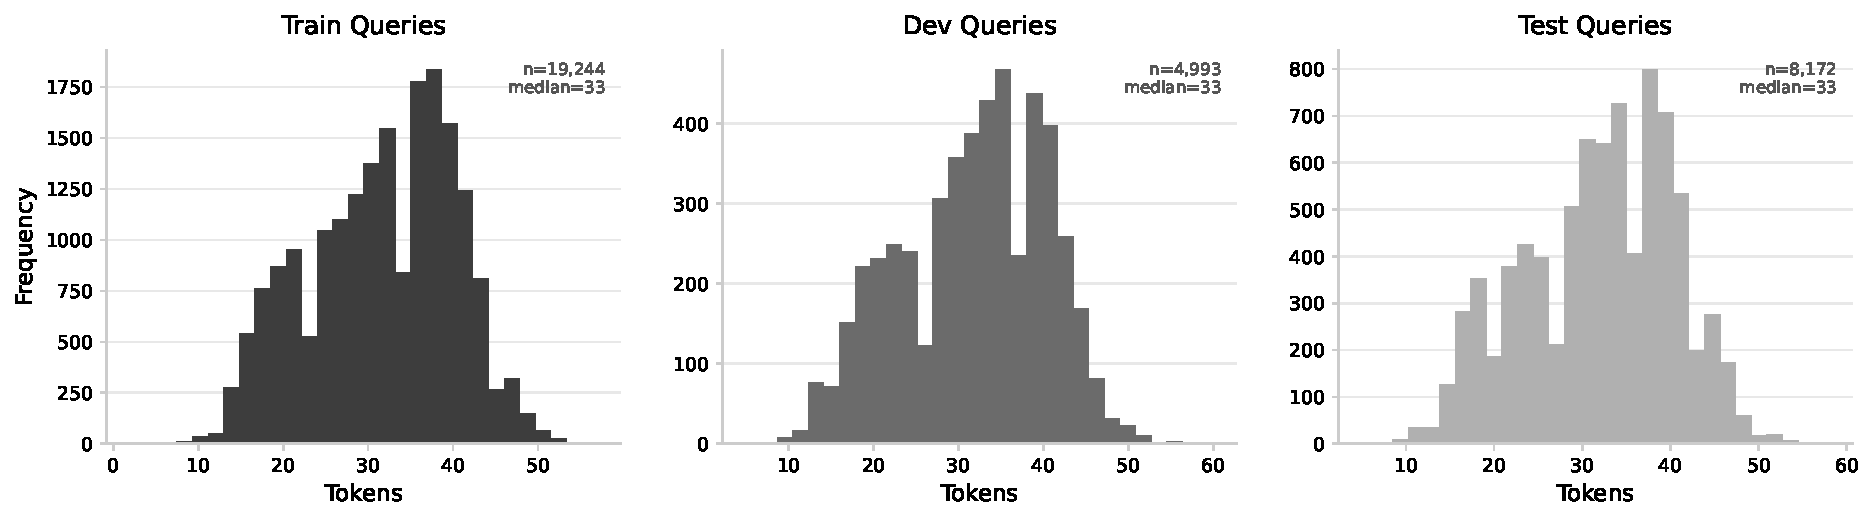
\includegraphics[width=1\linewidth]{figure/query_token_lengths.pdf}
	\caption{Train, dev and test datasets' distribution of query token length. }
	\label{fig:query_token_length_distribution}
\end{figure}